\chapter{Concepto de red de suminsitro}
%\section{Introducción: objetivos de aprendizaje y recursos}
\section{Concepto de red y cadena de suminsitro. Flujos y actores}
Una cadena / red de suminsitro es una red de organizaciones involucradas de manera directa o indirecta en la satisfacción de un pedido cliente-consumidor. 

Los actores que intervienen en una red de suministro ``tipo'' son:
\begin{itemize}
    \item clientes finales
    \item minoristas
    \item distribuidores
    \item fabricantes
    \item proveedores
    \item transportistas
    \item servicios,...
\end{itemize}

Es la secuencia integrada de procesos desde la adquisición de materias primas, su transformación en productos o servicios, su distribución hasta el consumidos final y su recirculación, así como la planificación integrada de todos ellos. Comprende los flujos coodinados de materiales, información y financieros desde los proveedores iniciales hasta los clientes finales.

En el conjunto y dentro de cada organización, la cadna de suministro afecta a todas las funciones necesarias para completar un pedido del cliente-consumidos (desarrollo del producto, marketing, operaciones, distribución, finanzas, servicio al cliente...).

\section{Tipos de decisiones en redes de suministro}
\begin{figure}[h]
    \centering
    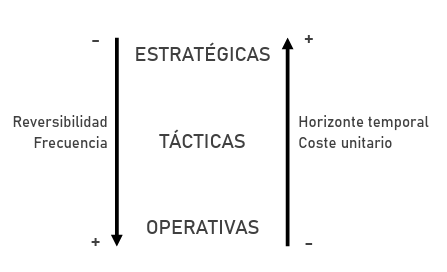
\includegraphics[width = 0.5 \textwidth]{Imagenes/Tema 1. Decisiones RS.png}
\end{figure}

\paragraph{Diseño / Estrategia.} Decisiones sobre la estructura y los procesos que se llevarán a cabo en la red de suministro. Decisiones de carácter estratégico:
\begin{itemize}
    \item Tipos de productos a fabricar
    \item Tecnologías
    \item Capacidad de plantas
    \item Localización de Instalaciones
    \item Distribución en plantas
    \item Modos de transporte
    \item Sistemas de información
\end{itemize}

\paragraph{Planificación.} Políticas que se van a llevar a cabo para las operaciones a corto/medio plazo. Decisiones de planificación:
\begin{itemize}
    \item Qué se suministrará a los mercados
    \item Desde dónde se suminsitrará (qué planta, qué centro, etc.)
    \item Políticas de inventarios
    \item Políticas de compras
    \item Periodos y dimensión de campañas de promoción
\end{itemize}

\paragraph{Operación.} La configuración de la cadena de suminsitro está ya fijada y las políticas de actuación también están definidas. El objetivo es implementar las políticas de operaciones de la forma más eficaz y eficiente posible. El horizonte temporal es la semana o el día. Los objetivos sobre los que tomar decisiones son pedidos individuales de clientes (no tipos de productos, ni productos). Al ser decisiones a muy corto plazo, se reduce mucho la incertidumbre. Ejemplos de decisiones operativas:
\begin{itemize}
    \item Colocar/confeccionar pedidos en almacenes
    \item Asignar pedidos en producción
    \item Agrupar pedidos por fechas/cliente
    \item Enviar pedidos:rutas
    \item Hacer reposiciones
    \item Medir resultados
    \item Adoptar medidas correctoras
\end{itemize}

\section{Enfoque de procesos en una red de suministro}
\subsection{Ciclo pedido-entrega; otros ciclos}
Los procesos en una red de suminsitro se dividen en ciclos. Cada ciclo se ejecuta en la interfaz entre dos etapas sucesivas de la cadena de suministro.
\begin{itemize}
    \item ciclo pedido del cliente
    \item ciclo de reaprovisionamiento
    \item ciclo de fabricación
    \item ciclo de aprovisionamiento
\end{itemize}

\subsection{Enfoques to order y to stock}
Los procesos en una red de suministro se dividen en dos categorías (\textit{to order} o \textit{to stock}) dependiendo de si los procesos responden a un pedido del cliente (enfoque \textins{to order}); o se trabaja de acuerdo a previsiones de pedidios de clientes (enfoque \textit{to stock}).

\begin{figure*}[h]
    \centering
    \begin{subfigure}[c]{0.45 \textwidth}
        \centering
        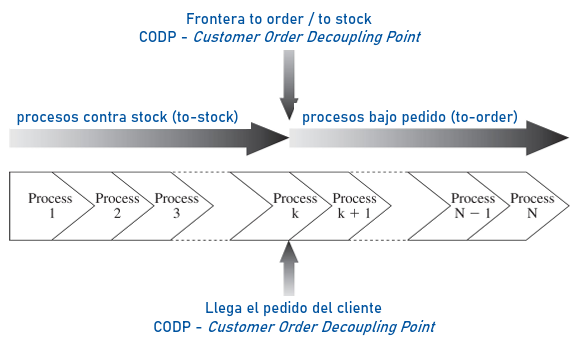
\includegraphics[width = \textwidth]{Imagenes/Tema 1. To order to stock (1).png}
    \end{subfigure}
    \begin{subfigure}[c]{0.45 \textwidth}
        \centering
        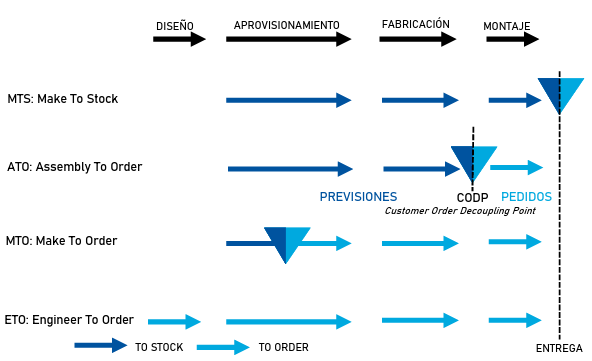
\includegraphics[width = \textwidth]{Imagenes/Tema 1. To order to stock (2).png}
    \end{subfigure}
\end{figure*}
